\chapter{CubeSatdesign}
Für die Realisierung einer ADR-Mission liegt der Fokus zunächst bei dem Entwurf eines geeigneten CubeSats. Infolgedessen wird in diesem Kapitel ein bestehendes Konzept \cite{Lettau.} anhand der Software QuSAD (SQL-Based CubeSat Analyse and Design Tool QuSAD) analysiert und gegebenenfalls optimiert. Zuvor wird ein Einblick in das Programm gegeben und durch eine anschließende Beschreibung des angenommenen Entwurfs erfolgt abschließend die Budgetplanung. Letztlich wird mittels der Budgets eine Auswertung des Designs bezüglich seiner Effizienz durchgeführt. Bei Bedarf werden Verbesserungen in Erwägung gezogen. Demnach kann ein zielführendes Missionsdesign bestimmt und bewertet werden.
		\section{QuSAD}
			\subsection{Einführung in die Software}
Die Software QuSAD (SQL-Based CubeSat Analyse and Design Tool) besteht aus einem SQL-Segment und einem MatLab Segment. Die SQL-Datenbank ist die Haupteingabequelle für das Entwerfen eines CubeSats und kategorisiert die CubeSat-Komponenten. Durch die wissenschaftliche Version können die COTS-Komponenten mit vordefinierten Parametern eingepflegt werden. Des Weiteren können auch individuelle Komponenten mit veränderbaren Parametern mittels der praxis Version hinzugefügt werden. Für das Abrufen der Komponententabelle aus der SQL-Datenbank wird MatLab verwendet. Dies wird durch mehrere grafische Benutzeroberflächen (GUI) realisiert und ermöglicht dem Benutzer eigene Satellitenzusammenstellungen. Neben dem CubeSat Design können Budget Analysen von Masse, Volumen, Energie, Preis und Verlinkung durch zur Verfügung stehenden Werkzeuge erstellt werden, um folglich eine Optimierung des Entwurfs zu ermöglichen. \cite{} \\
Für ein vertieftes Verständnis der Software wird auf das QuSAD-Handbuch \cite{} verwiesen. Das Anwendungsspektrum von QuSAD umfasst das erstellen eines Satelliten, sowie eine Bereitstellung einer Datenbank von Subsystemen für wissenschaftliche und auch lehrende Aspekte. Lehrende Aspekte umfassen den Einsatz der praktischen Version an Universitäten zur Unterstützung und Visualisierung. \cite{}
			\subsection{Datenbankerweiterung}
			Zur Erweiterung der Datenbank wird anfänglich die Auswahl der CubeSat-Komponenten einer ausgewählten Systemzusammenstellung verwendet (Siehe \tab{..}). Zu den besagten Komponenten werden alle bekannten Werte der Datenbank hinzugefügt. Des Weiteren müssen Recherchen bezüglich weiterer Herstellerangaben durchgeführt werden. Im Fokus liegen dabei alle Parameter die für die Budgetsplanungen benötigt werden. Angesichts der Budgetanalyse des zusammengestellten Satelliten wird eine Optimierung einiger COTS-Komponenten vorgenommen und dementsprechend die Datenbank um weitere Subsysteme erweitert. Zur Unterstützung der Ergänzungen wird eine interne Datenbank genutzt. Diese wurde von Mitarbeitern des Institutes Raumfahrtsysteme der Technischen Universität Braunschweig erstellt. Überwiegend sind die aufgelisteten Systeme mit einem TRL Wert hinterlegt. Da in vielen Fällen nur erprobte Systeme zum Einsatz kommen, werden Komponenten mit einem TRL Wert von 9 mit in die Datenbank hinzugefügt. Zusätzlich sind Internet-Quellenverweise (URL - Uniform Resource Locator) zu den meisten Einträgen vorhanden, über die man häufig direkt oder indirekt auf Datenblätter weitergeleitet wird und an weitere Informationen bezüglich des Subsystems gelangt.
			\subsection{Problematiken}
			Die Datenbankerweiterung und Budgeterstellung führte zu einigen Schwierigkeiten. Bei dem Laden der Datenbank über den SQL Server traten Fehlermeldungen bei MatLab auf, die nicht behoben werden konnten. Die Ursache könnte an der Inkompatibilität zwischen den neuen MatLab Versionen und MySQL liegen, da QuSAD mit der MatLab Version R2014 erstellt wurde. Im QuSAD Handbuch wird auf dieses Problem hingewiesen. Infolgedessen wurde die Datenbank über MySQL importiert und Lokal darauf zugegriffen. Die Datenbank wird in Mat-File Dateien gespeichert und kann über MatLab aufgerufen werden. Anschließend können die Komponenten in die gespeicherte Datenbank eingepflegt und als Workspace gesichert werden. Durch das Exportieren der neuen Datenbank über MySQL wird der Zugriff künftig bereitgestellt. Besonders problematisch gestaltete sich das einpflegen der Komponenten in die Datenbank. Im Handbuch, sowie den weiteren Dokumenten zur Datenbank wurde der Vorgang nicht hinreichend genau beschrieben. Des Weiteren gab es viele unbekannte Angaben über die hinzugefügten Komponenten. Diese mussten einzeln recherchiert und in seltenen fällen abgeschätzt werden. In der bereitgestellten Datenbank vom Institut fehlten an wichtigen Daten für die Budgets in den meisten fällen nur die Preise. Außerdem wurde festgestellt, dass einige URLs nicht mehr Gültig sind.
		\section{CubeSat- Designanalyse}
				\subsection{Angenommenes Design}
						%Hier die Varainte von Max nehmen und kurz beschreiben
				\subsection{Budgetplanung}
				
						\subsubsection{Massenbudget}
								
										\begin{figure}[h]
											\centering
												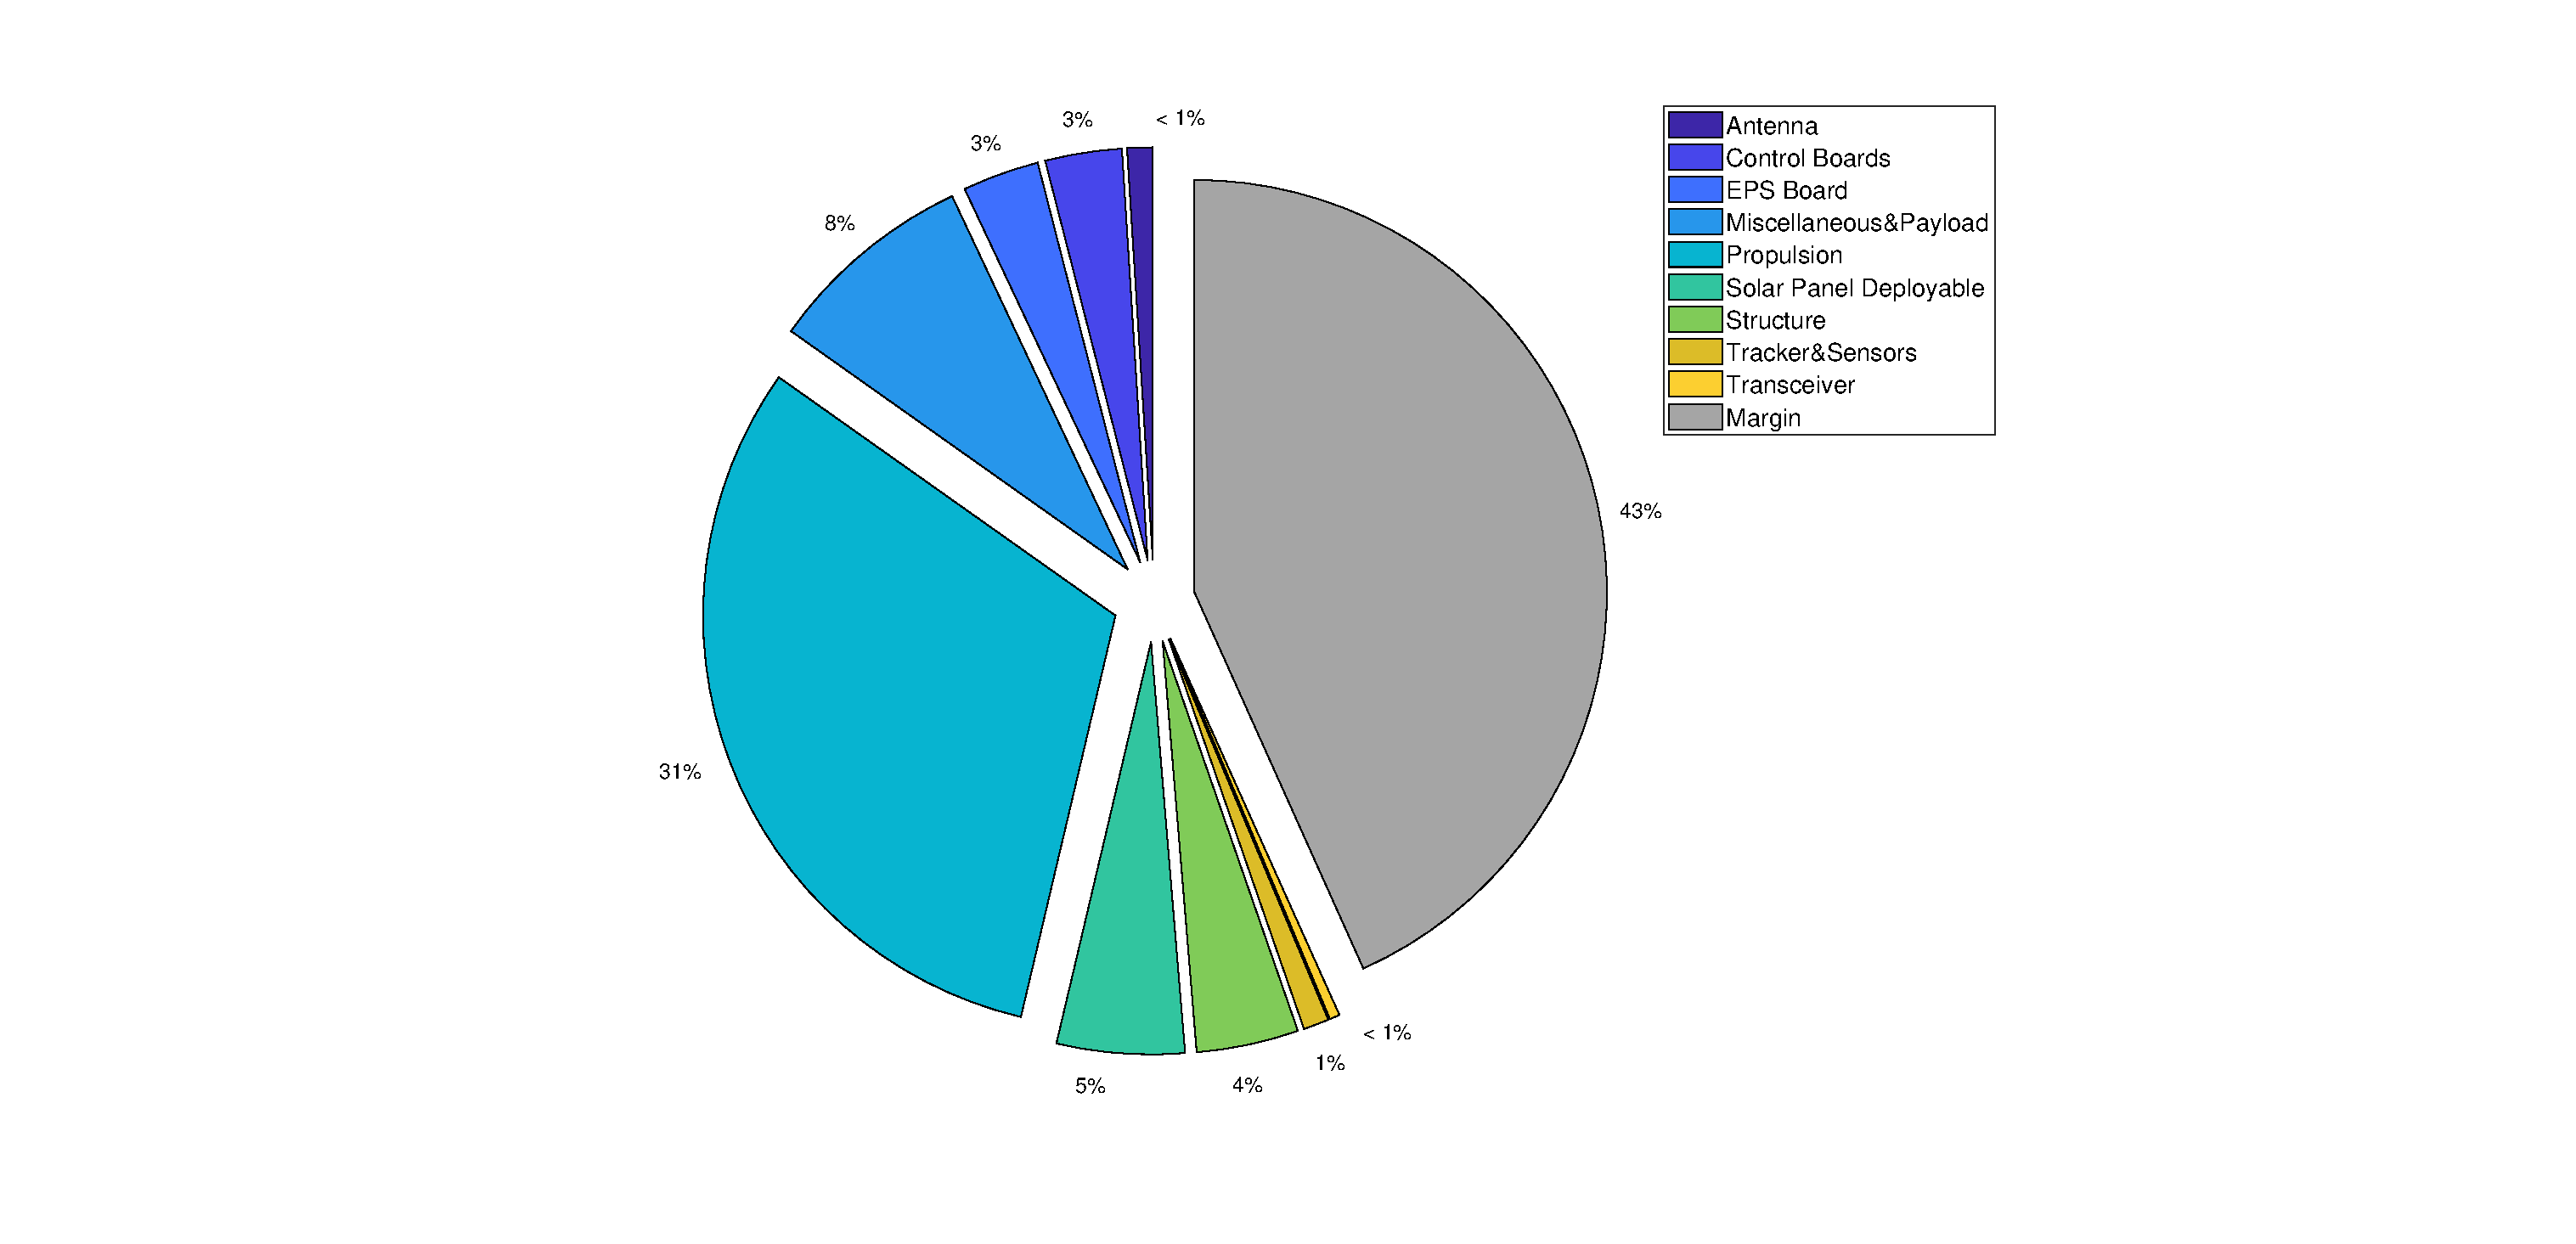
\includegraphics[width=0.60\textwidth]{masse}
											\caption{Massenbudget für das angenommene Design}
											\label{fig:masse}
										\end{figure}
										
						\subsubsection{Volumenbudget}
								
										\begin{figure}[h]
											\centering
												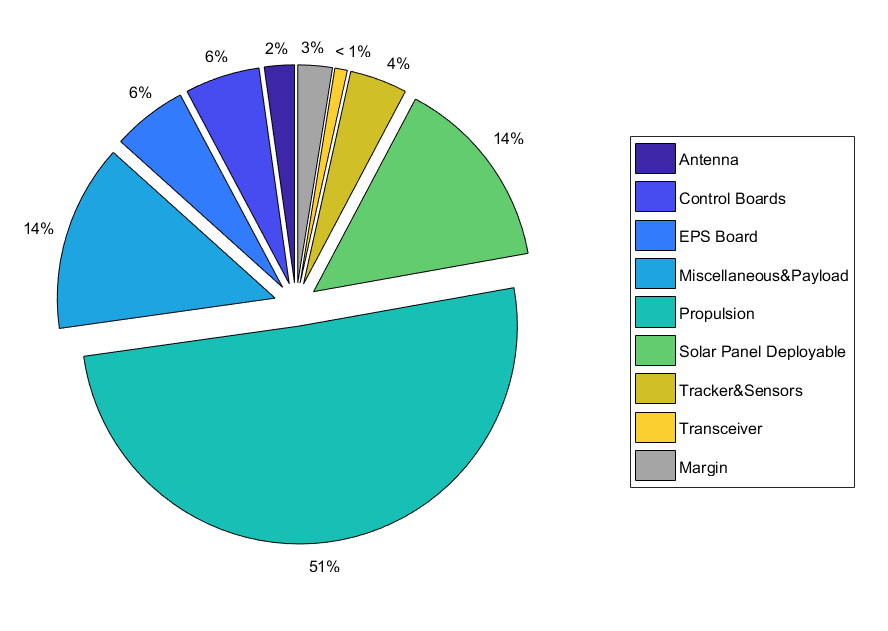
\includegraphics[width=0.60\textwidth]{volume}
											\caption{Volumenbudget für das angenommene Design}
											\label{fig:volume}
										\end{figure}
								
						\subsubsection{Leistungsbudget}
				
										\begin{figure}[h]
											\centering
												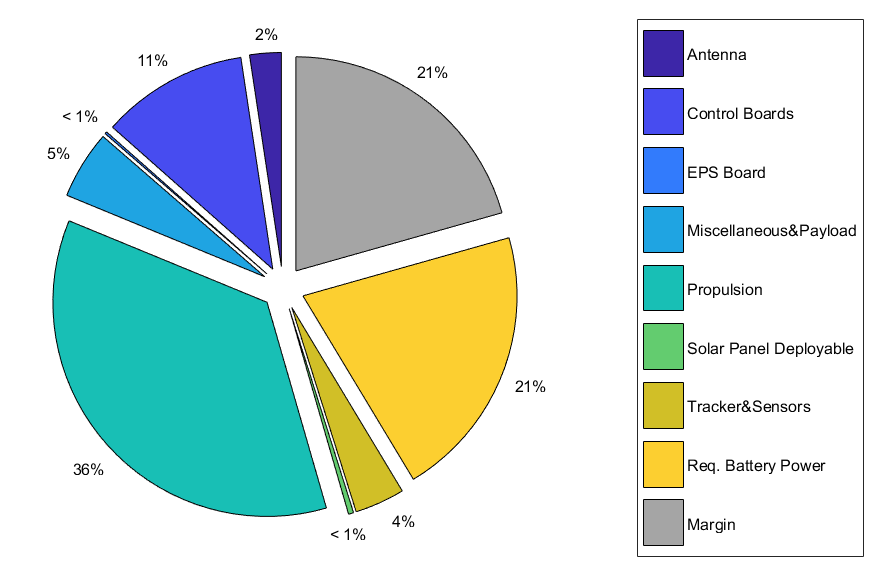
\includegraphics[width=0.60\textwidth]{power}
											\caption{Energiebudget für das angenommene Design}
											\label{fig:volume}
										\end{figure}
										
			\section{Auswertung und Optimierung des Designs}

				
